\flushleft
\chapter{Table-Driven Lexer}
\section{Specification : micro-syntax}

\textbf{Task:} Identify rules (micro-syntax) to validate if a sequence of characters is a \emph{lexeme} (the smallest lexical unit allowed in the language).

\vskip 0.2in

We can construct infinite number of lexemes (e.g.  $\mathbb{Z}$). To gain control, we categorise the lexemes into a finite number of groups and then write rules for each group to verify if a sequence of characters is a \emph{lexeme} in the group.

\vskip 0.2in

The task of choosing groups/types is not deterministic; however, a typical strategy (and the one used in this implementation) is:

\begin{itemize}
    \item Place keywords (reserved/special words in the language) in separate groups:
        \begin{table}[H]
        \scriptsize
        \centering
        \begin{tabular}{c c}
            Group & Lexeme(s) \\
            \hline
            \verb!TOK_PRINT! & \verb!print! \\
            \verb!TOK_IF! & \verb!if! \\
            \verb!TOK_ELSE! & \verb!else! \\
            \verb!TOK_FOR! & \verb!for! \\
            \verb!TOK_WHILE! & \verb!while! \\
            \verb!TOK_FN! & \verb!fn! \\
            \verb!TOK_RETURN! & \verb!return! \\
            \verb!TOK_INT_TYPE! & \verb !while! \\
            \verb!TOK_FLOAT_TYPE! & \verb!float! \\
            \verb!TOK_BOOL_TYPE! & \verb!bool! \\
            \verb!TOK_CHAR_TYPE! & \verb!char! \\
            \verb!TOK_LET! & \verb!let! \\
            \verb!TOK_RIGHT_ARROW! & \verb!->! \\
        \end{tabular}
        \caption{Keywords and their respective group.}
        \label{tab: keyword lexemes}
    \end{table}
    \item Similarly, place punctuation symbols in separate groups: 
    \begin{table}[H]
        \small
        \centering
        \begin{tabular}{c|c}
            Group & Lexeme(s) \\
            \hline
            \verb!TOK_LEFT_ROUND_BRACKET! & \verb!(! \\
            \verb!TOK_RIGHT_ROUND_BRACKET!! & \verb!)! \\
            \verb!TOK_LEFT_CURLY_BRACKET! & \verb!{! \\
            \verb!TOK_RIGHT_CURLY_BRACKET! & \verb!}! \\
            \verb!TOK_COMMA! & \verb!,! \\
            \verb!TOK_COLON! & \verb!:! \\
            \verb!TOK_SEMICOLON! & \verb!;! \\
        \end{tabular}
        \caption{Different punctuation symbols and their respective group:}
        \label{tab:punctuation lexemes}
    \end{table}
    \item Put operators of similar type into one group (we categorise them according to EBNF spec): 
    \begin{table}[H]
    \small
    \centering
    \begin{tabular}{c|c}
        Group and Lexeme(s) \\
        \hline
        \verb!TOK_MULTIPLICATIVE_OP! & \verb!'*'|'/'|'and'! \\
        \verb!TOK_ADDITIVE_OP! & \verb!'+'|'-'|'or'! \\
        \verb!TOK_RELATIONAL_OP! & \verb!'<' | '>' | '==' | '!=' | '<=' | '>=' ! \\
    \end{tabular}
      \caption{Different operations and their respective group}
    \label{tab:operation lexemes}
    \end{table}
    \item Group identifiers (of variables/functions) into one group and group literals by their respective data type. 
        \begin{table}[H]
        \small
        \centering
        \begin{tabular}{c|c}
        TokenType & Lexeme(s) \\
        \hline 
           \verb!TOK_IDENTIFIER!  & \verb!( '_' | <Letter> ) ( '_' | <Letter> | <Digit>)*!  \\
           \verb!TOK_BOOLEAN_LITERAL! & \verb!'true' | 'false'!  \\
           \verb!TOK_INTEGER_LITERAL! & \verb!<Digit>{<Digit>}! \\
           \verb!TOK_FLOAT_LITERAL! & \verb!<Digit>{<Digit>}.<Digit>{<Digit>}! \\
           \verb!TOK_CHAR_LITERAL! & \verb!'‘' <Printable> '’'! \\
        \end{tabular}
        \caption{Tokens and their respective group(s)}
        \label{tab:identifier literals lexemes}
    \end{table}
    \item Special lexemes : 
    \begin{table}[H]\
        \footnotesize
        \centering
        \begin{tabular}{c|c}
        TokenType & Lexeme(s) \\
        \hline 
           \verb!TOK_SKIP!  & \verb!whitespace characters | //{<printable>} \n  |  /*{<printable>}*/! \\
             \verb!TOK_EOF!  & \verb!EOF! 
        \end{tabular}
        \caption{Special lexemes and their respective group(s)}
        \label{tab:special lexemes}
    \end{table}   
\end{itemize}

Having all the possible groups in hand, we can construct an automaton capturing tinylang's syntax by designing sub-automata for each group and then merging the automata together at the starting state.

\subsection{Constructing a deterministic finite-state automaton (DFSA) that recognises all possible lexemes}

Let $G$ be the set consisting of all groups described in Tables \ref{tab: keyword lexemes}, \ref{tab:punctuation lexemes}, \ref{tab:operation lexemes}, \ref{tab:identifier literals lexemes}, and \ref{tab:special lexemes}, and let ll represent some lexeme.

\vskip 0.2in 



We note that groups \textbf{should} partition the set of all lexemes.

\begin{itemize}
    \item All groups cover all possible lexemes in tinylang: $  \bigcup\limits_{g \in G} \{  l  : l \in g  \}$ is the set of all possible lexemes.
    \item Pairwise disjoint: $\forall g_1,g_2 \in G \implies g_1 \cap g_2 = \phi$
\end{itemize}

\noindent\textbf{NB: } The specification of the groups described in Tables \ref{tab: keyword lexemes}, \ref{tab:punctuation lexemes}, \ref{tab:operation lexemes}, \ref{tab:identifier literals lexemes} and \ref{tab:special lexemes} contradicts the pairwise disjoint property since there exist clashes, for example, lexeme \verb!if!  can be in both groups \verb!TOK_IDENTIFIER! and \verb!TOK_IF!. In this case, priority is trivially given to the group \verb!TOK_IF!.  During the design stage, attention is given to these types of non-disjoint clashes to ensure that the groups partition the set of all possible lexemes.

\subsection{Design of the sub-automata}

\subsubsection{Important consideration}

We want the sub-automata to be deterministic finite-state automata:

\begin{itemize}
    \item \textbf{Deterministic} : Given a state and input, we deterministically know what the next state is (i.e., given a state and input, there are no two distinct transitions taking us to different states). 
    \item \textbf{Finite} : Gives us a handle on all possible lexemes in a group.
\end{itemize}

\vskip 0.2in
\subsubsection{Classifier Table}
While sketching the automata on pen and paper and  keeping in mind the EBNF rules equivalent inputs used for the sub-automata where classified as follows:
\begin{table}[H]
\small
\centering
\begin{tabular}{|l|l|l|}
\hline
\rowcolor[HTML]{FE0000} 
Input & Value(s) & \begin{tabular}[c]{@{}l@{}}ASCII-\\ EQUIVALENT\end{tabular} \\ \hline
letter & a,b,...,z,A,B,..,Z & {[}0x4a0x5a{]},{[}0x61,0x7a{]} \\ \hline
digit & 0,1,2,...,9 & {[}0x30,0x39{]} \\ \hline
\_ & \_ & 0x5f \\ \hline
/ & / & 0x2f \\ \hline
* & * & 0x2a \\ \hline
\textless{} & \textless{} & 0x3c \\ \hline
+ & + & 0x2b \\ \hline
- & - & 0x2d \\ \hline
= & = & 0x3d \\ \hline
! & ! & 0x21 \\ \hline
. & . & 0x2e \\ \hline
\Verb!'! & \Verb!'! & 0x27 \\ \hline
\Verb!punct! &( ) , : ; \{ \}  & $\{\text{0x28, 0x29, 0x2c, 0x3a, 0x3b, 0x7b, 0x7d}\}$ \\ \hline
\begin{tabular}[c]{@{}l@{}}other\_\\ printable\end{tabular} & space,...,$\sim$ & \begin{tabular}[c]{@{}l@{}}{[}0x20,0x7e{]} excluding the ASCII codes\\ above\end{tabular} \\ \hline
\end{tabular}
\caption{Classifier table}
\label{table:classifier table}
\end{table}
\textbf{Note: } All the input categories are pairwise disjoint. This ensures that the automata are deterministic.




\textbf{Also note: } In the following sub-automata shown in figures \ref{fig: char literals automata}, \ref{fig:identifier and keywords automaton}, \ref{fig: comments and multiline comments automaton}, \ref{fig: punctatuation automaton}, \ref{fig: int float automaton} and \ref{fig: additive op relative op automata} input \verb!any! is an abbreviation for:


\verb@letter|digit|'_'|'/'|'*'|'<'|'>'|'+'|'-'|'='|'!'|'.'|'@
\verb@|punct|other_printable@ i.e. all the printable characters allowed in tinylang given by ASCII range \verb![0x20-0x7e]! (see section \ref{sec:ebnf-tinylang-rules}).
\vskip 0.2in

We start considering different groups:
\begin{itemize}
    \item Group \verb!TOK_CHAR_LITERAL!
    \begin{figure}[H]
        \centering
            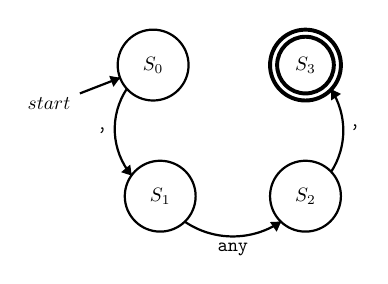
\begin{tikzpicture}[thick,scale=0.15, every node/.style={scale=0.7}]
            \tikzstyle{every node}+=[inner sep=0pt]
            \draw [black] (27.1,-28.6) circle (3);
            \draw (27.1,-28.6) node {$S_0$};
            \draw [black] (27.7,-39.7) circle (3);
            \draw (27.7,-39.7) node {$S_1$};
            \draw [black] (40,-39.7) circle (3);
            \draw (40,-39.7) node {$S_2$};
            \draw [line width = 0.5mm,black] (40,-28.6) circle (3);
            \draw (40,-28.6) node {$S_3$};
            \draw [line width = 0.5mm,black] (40,-28.6) circle (2.4);
            \draw [black] (20.9,-31) -- (24.3,-29.68);
            \draw (20.15,-31.85) node [left] {$start$};
            \fill [black] (24.3,-29.68) -- (23.38,-29.51) -- (23.74,-30.44);
            \draw [black] (25.292,-37.962) arc (-139.85174:-213.96015:6.127);
            \fill [black] (25.29,-37.96) -- (25.16,-37.03) -- (24.39,-37.67);
            \draw (23.28,-34.37) node [left] {\verb!'!};
            \draw [black] (37.937,-41.848) arc (-55.6929:-124.3071:7.251);
            \fill [black] (37.94,-41.85) -- (36.99,-41.89) -- (37.56,-42.71);
            \draw (33.85,-43.61) node [below] {\verb!any!};
            \draw [black] (42.159,-30.644) arc (33.15644:-33.15644:6.411);
            \fill [black] (42.16,-30.64) -- (42.18,-31.59) -- (43.01,-31.04);
            \draw (43.7,-34.15) node [right] {\verb!'!};
            \end{tikzpicture}
            \caption{dfsa recognising lexemes in group \emph{TOK\_CHAR\_LITERAL}}
            \label{fig: char literals automata}
    \end{figure}
    \begin{itemize}
  
        \item  Sequences of characters leading to state 3 are lexemes in group \verb!TOK_CHAR_LITERAL!.
        \item Sequences of characters leading to States 0, 1 and 2 are invalid
        \item   \textbf{NB : } This automata only capture lexeme(s) that are in group
        \verb!TOK_CHAR_LITERAL! (i.e. no non-disjoint clashes).
    \end{itemize}
    
  
    \item Group \verb!TOK_IDENTIFIER! :
    \begin{figure}[H]
        \centering
        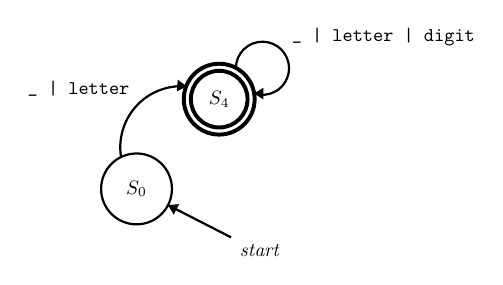
\begin{tikzpicture}[thick,scale=0.15, every node/.style={scale=0.7}]
            \tikzstyle{every node}+=[inner sep=0pt]
            \draw [black] (26.2,-33.9) circle (3);
            \draw (26.2,-33.9) node {$S_0$};
            \draw [line width = 0.5mm, black] (33.2,-26.3) circle (3);
            \draw (33.2,-26.3) node {$S_4$};
            \draw [line width = 0.5mm, black] (33.2,-26.3) circle (2.4);
            \draw [black] (34.2,-38) -- (28.87,-35.27);
            \draw (34.89,-39.13) node [right] {\emph{start}};
            \fill [black] (28.87,-35.27) -- (29.35,-36.08) -- (29.81,-35.19);
            \draw [black] (24.895,-31.245) arc (-170.40794:-274.88546:5.183);
            \fill [black] (30.45,-25.22) -- (29.69,-24.65) -- (29.61,-25.65);
            \draw (25.66,-25.41) node [left] {\verb!_ | letter!};
            \draw [black] (34.612,-23.666) arc (179.53768:-108.46232:2.25);
            \draw (39.28,-21) node [right] {\verb!_ | letter | digit!};
            \fill [black] (36.15,-25.82) -- (36.95,-26.33) -- (36.95,-25.33);
        \end{tikzpicture}
        \caption{dfsa recognising lexemes in group \emph{TOK\_IDENTIFIER}}
        \label{fig:identifier and keywords automaton}
    \end{figure}
    
    \textbf{NB : } This automaton also recognises lexemes that are in groups: \verb!TOK_LET!, \verb!TOK_IF!, \verb!TOK_ELSE!, \verb!TOK_FOR!, \verb!TOK_WHILE!, \verb!TOK_RETURN!, \verb!TOK_INT_TYPE!, \verb!TOK_FLOAT_TYPE!, \verb!TOK_BOOL_TYPE!, \verb!TOK_CHAR_TYPE! and \verb!TOK_BOOLEAN_LITERAL!. We give precedence to these groups i.e. if a lexeme that is identified by this automaton  is in one of these groups we consider it that it is in that group not in group \verb!TOK_IDENTIFIER! (in simpler terms an identifier cannot be a reserved word). Note that these keyword groups can be given the same precedence since they are all pairwise disjoint.
    \item Group \verb!TOK_SKIP! :
    \begin{itemize}
        \begin{figure}[H]
            \centering
            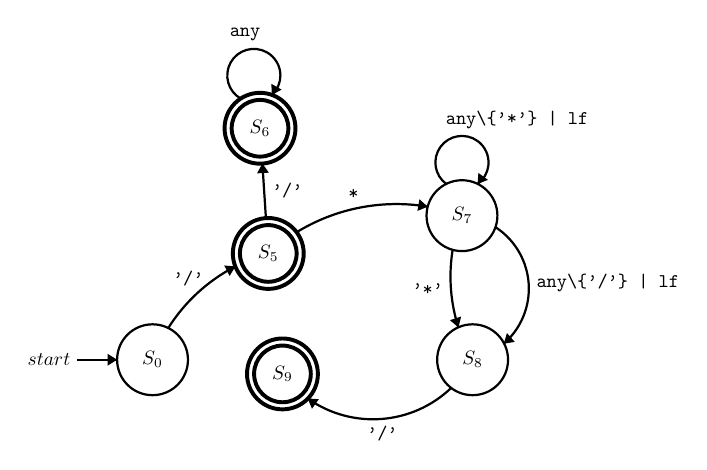
\begin{tikzpicture}[thick,scale=0.15, every node/.style={scale=0.7}]
            \tikzstyle{every node}+=[inner sep=0pt]
                \draw [black] (24.7,-28.4) circle (3);
                \draw (24.7,-28.4) node {$S_0$};
                \draw [line width = 0.5mm,line width = 0.5mm,black] (34.5,-19.4) circle (3);
                \draw (34.5,-19.4) node {$S_5$};
                \draw [line width = 0.5mm,black] (34.5,-19.4) circle (2.4);
                \draw [line width = 0.5mm, black] (33.8,-8.8) circle (3);
                \draw (33.8,-8.8) node {$S_6$};
                \draw [line width = 0.5mm, black] (33.8,-8.8) circle (2.4);
                \draw [black] (50.9,-16.2) circle (3);
                \draw (50.9,-16.2) node {$S_7$};
                \draw [black] (51.8,-28.4) circle (3);
                \draw (51.8,-28.4) node {$S_8$};
                \draw [line width = 0.5mm,black] (35.7,-29.6) circle (3);
                \draw (35.7,-29.6) node {$S_9$};
                \draw [line width = 0.5mm,black] (35.7,-29.6) circle (2.4);
                \draw [black] (18.3,-28.4) -- (21.7,-28.4);
                \draw (17.8,-28.4) node [left] {$start$};
                \fill [black] (21.7,-28.4) -- (20.9,-27.9) -- (20.9,-28.9);
                \draw [black] (26.03,-25.717) arc (147.79095:117.33575:14.69);
                \fill [black] (31.71,-20.5) -- (30.77,-20.42) -- (31.23,-21.31);
                \draw (27.73,-22.24) node [above] {\verb!'/'!};
                \draw [black] (34.3,-16.41) -- (34,-11.79);
                \fill [black] (34,-11.79) -- (33.55,-12.62) -- (34.55,-12.56);
                \draw (34.75,-14.06) node [right] {\verb!'/'!};
                \draw [black] (32.175,-6.292) arc (240.66765:-47.33235:2.25);
                \draw (32.53,-1.42) node [above] {\verb!any!};
                \fill [black] (34.8,-5.98) -- (35.63,-5.53) -- (34.76,-5.04);
                \draw [black] (36.898,-17.604) arc (121.51467:80.56721:16.174);
                \fill [black] (48,-15.44) -- (47.3,-14.81) -- (47.13,-15.8);
                \draw (41.71,-14.93) node [above] {\verb!*!};
                \draw [black] (49.577,-13.52) arc (234:-54:2.25);
                \draw (50.9,-8.95) node [above,xshift=1cm] {\verb!any\{'*'} | lf!};
                \fill [black] (52.22,-13.52) -- (53.1,-13.17) -- (52.29,-12.58);
                \draw [black] (50.595,-25.659) arc (-162.33655:-189.22526:14.168);
                \fill [black] (50.6,-25.66) -- (50.83,-24.74) -- (49.88,-25.05);
                \draw (49.36,-22.45) node [left] {\verb!'*'!};
                \draw [black] (53.712,-17.158) arc (57.31408:-48.87589:6.196);
                \fill [black] (54.44,-27.04) -- (55.37,-26.89) -- (54.71,-26.14);
                \draw (57.15,-21.87) node [right] {\verb!any\{'/'} | lf !};
                \draw [black] (49.993,-30.779) arc (-46.20359:-125.27119:9.572);
                \fill [black] (37.84,-31.68) -- (38.2,-32.55) -- (38.78,-31.74);
                \draw (44.16,-33.97) node [below] {\verb!'/'!};
            \end{tikzpicture}
            \caption{dfsa recognising lexemes in group \emph{TOK\_SKIP}}
            \label{fig: comments and multiline comments automaton}
        \end{figure}
        \item Since the input \verb!'/'! is utilised to identify a lexeme in group \verb!TOK_SKIP!, the same automaton can capture lexeme \verb!'/'! in group \verb!TOK_MULTIPLICATIVE_OP! (this ensures that when we merge the sub-automata the main automaton remains determinstic).
        \item Sequence of character(s) leading to state 5 is lexeme in group \verb!TOK_MULTIPLICATIVE_OP!. Sequence of character(s) leading to states 6 and 9 are lexemes in group \verb!TOK_SKIP!.
        \item Sequence of character(s) leading to states 0,7 and 8 are invalid.
    \end{itemize}
    \item Groups \verb!TOK_LEFT_ROUND_BRACKET!, \verb!TOK_RIGHT_ROUND!, \verb!TOK_LEFT_CURLY_BRACKET!, \verb!TOK_RIGHT_CURLY_BRACKET!, \verb!TOK_COMMA!, \verb!TOK_COLON! and \verb!TOK_SEMICOLON! : 
    \begin{figure}[H]
        \centering
        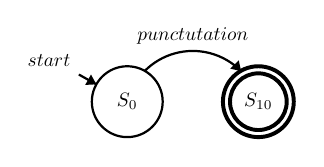
\begin{tikzpicture}[thick,scale=0.15, every node/.style={scale=0.7}]
            \tikzstyle{every node}+=[inner sep=0pt]
            \draw [black] (28.2,-20) circle (3);
            \draw (28.2,-20) node {$S_0$};
            \draw [line width = 0.5mm,black] (39.3,-20) circle (3);
            \draw (39.3,-20) node {$S_{10}$};
            \draw [line width = 0.5mm,black] (39.3,-20) circle (2.4);
            \draw [black] (24.1,-17.7) -- (25.58,-18.53);
            \draw (23.44,-16.49) node [left] {$start$};
            \fill [black] (25.58,-18.53) -- (25.13,-17.7) -- (24.64,-18.58);
            \draw [black] (29.66,-17.419) arc (135.51256:44.48744:5.733);
            \fill [black] (37.84,-17.42) -- (37.64,-16.5) -- (36.92,-17.2);
            \draw (33.75,-15.2) node [above] {$punctutation$};
        \end{tikzpicture}
        \caption{dfsa recognising lexemes in punctation groups}
        \label{fig: punctatuation automaton}
    \end{figure}
    \begin{itemize}
        \item Since no punctuation is used as an initial input (from starting state) in any of the other sub-automata we can simplify the automaton by capturing all the punctuation symbols in one state ensuring that the main automaton remains deterministic when merging.
        \item A checker function then checks what type of punctuation it is and matches it accordingly.
        \item We conclude that a character leading to state 10 is a lexeme in one of the following groups :  \verb!TOK_LEFT_ROUND_BRACKET!, \verb!TOK_RIGHT_ROUND!, \verb!TOK_LEFT_CURLY_BRACKET!, \verb!TOK_RIGHT_CURLY_BRACKET!, \verb!TOK_COMMA!, \verb!TOK_COLON! and \verb!TOK_SEMICOLON!.
    \end{itemize}
    \item Groups \verb!TOK_INT! and \verb!TOK_FLOAT!:
    \begin{figure}[H]
        \centering
        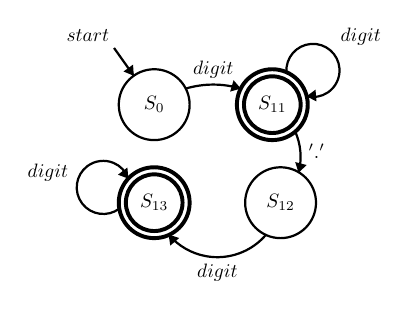
\begin{tikzpicture}[thick,scale=0.15, every node/.style={scale=0.7}]
        \tikzstyle{every node}+=[inner sep=0pt]
        \draw [black] (22.9,-14.4) circle (3);
        \draw (22.9,-14.4) node {$S_0$};
        \draw [line width = 0.5mm,black] (32.9,-14.4) circle (3);
        \draw [line width = 0.5mm,black] (32.9,-14.4) node {$S_{11}$};
        \draw [line width = 0.5mm,black] (32.9,-14.4) circle (2.4);
        \draw  [black] (33.6,-22.7) circle (3);
        \draw (33.6,-22.7) node {$S_{12}$};
        \draw [line width = 0.5mm,black] (22.9,-22.7) circle (3);
        \draw [line width = 0.5mm,black](22.9,-22.7) node {$S_{13}$};
        \draw [line width = 0.5mm,black] (22.9,-22.7) circle (2.4);
        \draw [black] (25.556,-13.041) arc (106.6108:73.3892:8.2);
        \fill [black] (30.24,-13.04) -- (29.62,-12.33) -- (29.33,-13.29);
        \draw (27.9,-12.2) node [above] {$digit$};
        \draw [black] (34.098,-11.662) arc (184.10091:-103.89909:2.25);
        \draw (38.61,-8.61) node [right] {$digit$};
        \fill [black] (35.8,-13.69) -- (36.64,-14.13) -- (36.56,-13.13);
        \draw [black] (34.826,-16.647) arc (24.32689:-14.68535:5.281);
        \fill [black] (35.12,-20.16) -- (35.81,-19.51) -- (34.84,-19.26);
        \draw (35.9,-18.32) node [right] {$'.'$};
        \draw [black] (32.379,-25.398) arc (-40.22898:-139.77102:5.409);
        \fill [black] (24.12,-25.4) -- (24.26,-26.33) -- (25.02,-25.69);
        \draw (28.25,-27.81) node [below] {$digit$};
        \draw [black] (19.953,-23.196) arc (307.28372:19.28372:2.25);
        \draw (15.67,-20.15) node [left] {$digit$};
        \fill [black] (20.71,-20.66) -- (20.63,-19.72) -- (19.83,-20.33);
        \draw [black] (19.5,-9.6) -- (21.17,-11.95);
        \draw (17.28,-9.1) node [above] {$start$};
        \fill [black] (21.17,-11.95) -- (21.11,-11.01) -- (20.3,-11.59);
        \end{tikzpicture}
        \caption{dfsa recognising lexemes in group \emph{TOK\_INT} and \emph{TOK\_FLOAT}}
        \label{fig: int float automaton}
    \end{figure}
    \begin{itemize}
        \item Sequences of characters leading to States 11 and 13 are in groups \verb!TOK_INT! and \verb!TOK_FLOAT! respectively.
        \item Sequences of characters leading to States 0 and 12 are invalid.
        \item \textbf{NB : } Since 12 is rejecting, floating points like $12.$, $0.$  \textbf{are not allowed } i.e. the fractional part must contain 1 or more digit. Example of good floating point numbers are $12.3, 432.124214$ etc. This strategy is taken since it conforms to the EBNF rules.
    \end{itemize}
    \item Groups \verb!TOK_ADDITIVE_OP!, \verb!MULTIPLICATIVE_OP!, \verb!TOK_RELATIONAL_OP! and \verb!TOK_RIGHT_ARROW! 
    \begin{figure}[H]
        \centering
        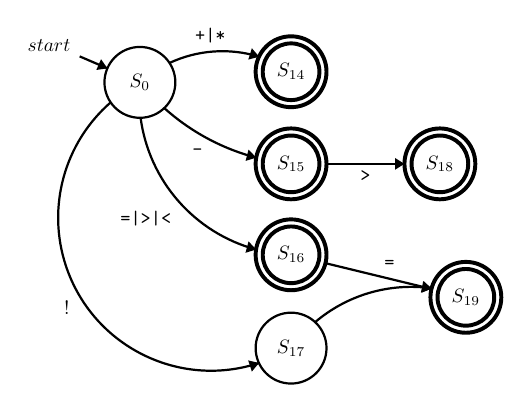
\begin{tikzpicture}[thick,scale=0.15, every node/.style={scale=0.7}]
\tikzstyle{every node}+=[inner sep=0pt]
\draw [black] (18,-14.2) circle (3);
\draw (18,-14.2) node {$S_0$};
\draw [line width = 0.5mm,black] (30.8,-13.3) circle (3);
\draw (30.8,-13.3) node {$S_{14}$};
\draw [line width = 0.5mm,black] (30.8,-13.3) circle (2.4);
\draw [line width = 0.5mm,black] (30.8,-21.1) circle (3);
\draw (30.8,-21.1) node {$S_{15}$};
\draw [line width = 0.5mm,black] (30.8,-21.1) circle (2.4);
\draw [line width = 0.5mm,black] (30.8,-28.8) circle (3);
\draw (30.8,-28.8) node {$S_{16}$};
\draw [line width = 0.5mm,black] (30.8,-28.8) circle (2.4);
\draw [black] (30.8,-36.7) circle (3);
\draw (30.8,-36.7) node {$S_{17}$};
\draw [line width = 0.5mm,black] (43.4,-21.1) circle (3);
\draw (43.4,-21.1) node {$S_{18}$};
\draw [line width = 0.5mm,black] (43.4,-21.1) circle (2.4);
\draw [line width = 0.5mm,black] (45.6,-32.4) circle (3);
\draw (45.6,-32.4) node {$S_{19}$};
\draw [line width = 0.5mm,black] (45.6,-32.4) circle (2.4);
\draw [black] (12.9,-12) -- (15.25,-13.01);
\draw (12.17,-11.04) node [left] {$start$};
\fill [black] (15.25,-13.01) -- (14.71,-12.24) -- (14.31,-13.15);
\draw [black] (20.5,-12.56) arc (115.13167:72.91231:10.57);
\fill [black] (28.1,-12.03) -- (27.48,-11.31) -- (27.18,-12.27);
\draw (23.97,-10.91) node [above] {\verb!+|*!};
\draw [black] (27.85,-20.573) arc (-104.70965:-131.94523:18.789);
\fill [black] (27.85,-20.57) -- (27.2,-19.89) -- (26.95,-20.85);
\draw (22.87,-19.44) node [below] {\verb!-!};
\draw [black] (27.84,-28.35) arc (-105.06596:-172.45116:13.374);
\fill [black] (27.84,-28.35) -- (27.2,-27.66) -- (26.94,-28.63);
\draw (20.72,-25.7) node [left] {\verb!=|>|<!};
\draw [black] (28.085,-37.96) arc (-71.73997:-228.9899:12.95);
\fill [black] (28.08,-37.96) -- (27.17,-37.74) -- (27.48,-38.69);
\draw (12.11,-33.29) node [left] {\verb!!!};
\draw [black] (33.8,-21.1) -- (40.4,-21.1);
\fill [black] (40.4,-21.1) -- (39.6,-20.6) -- (39.6,-21.6);
\draw (37.1,-21.6) node [below] {\verb!>!};
\draw [black] (33.72,-29.51) -- (42.68,-31.69);
\fill [black] (42.68,-31.69) -- (42.03,-31.02) -- (41.79,-31.99);
\draw (39.14,-30) node [above] {\verb!=!};
\draw [black] (32.833,-34.504) arc (130.36454:82.03691:12.559);
\fill [black] (42.71,-31.64) -- (41.98,-31.03) -- (41.84,-32.02);
\end{tikzpicture}
        \caption{dfsa recognising lexemes in groups all operator groups and  group \emph{TOK\_RIGHT\_ARROW}}
        \label{fig: additive op relative op automata}
    \end{figure}
    \begin{itemize}
        \item Sequences of characters leading to State 14 are in groups \verb!TOK_ADDITIVE_OP! or \verb!TOK_MULTIPLICATIVE_OP!. We use a checker function to check the operator and  assign the appropriate groups. Sequence of characters leading to State 15 are in group \verb!TOK_ADDITIVE_OP!. Sequences of characters leading to State 16 are in group \verb!TOK_RELATIONAL_OP!. Sequence of characters leading to State 17 is invalid. Sequence of characters leading to State 17 is in group \verb!TOK_RIGHT_ARROW!. Sequence of characters leading to State 19 are in group \verb!TOK_RELATIONAL_OP!.
        \item \textbf{NB} : The multiplicative op \verb!'/'! is already dealt with in automaton shown in figure \ref{fig: comments and multiline comments automaton}
    
    
    \end{itemize}


\end{itemize}
\vskip 2in
\subsection{tinylang Automaton}
Merging all the sub-automata in figures \ref{fig: char literals automata}, \ref{fig:identifier and keywords automaton}, \ref{fig: comments and multiline comments automaton}, \ref{fig: punctatuation automaton}, \ref{fig: int float automaton} and \ref{fig: additive op relative op automata} at the starting starting state we get the following 20-state dfsa that is able to deterministically recognise all the lexemes in tinylang and their respective groups (with the help of some extra helper function which will be discussed later).

\begin{figure}[H]
    \centering
    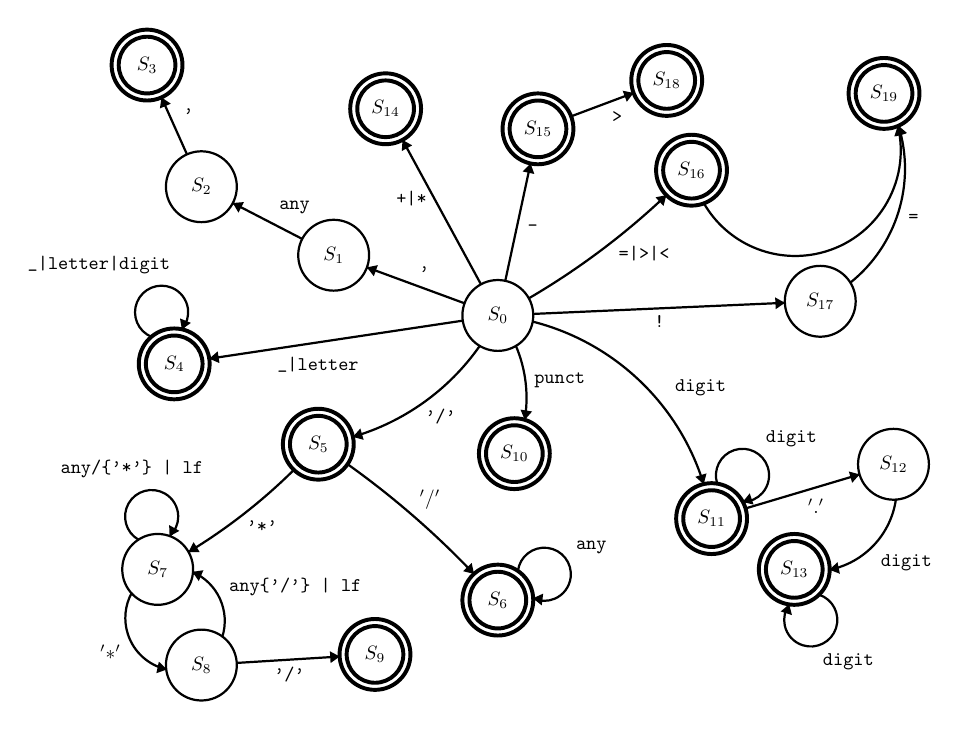
\begin{tikzpicture}[thick,scale=0.15, every node/.style={scale=0.7}]
    \tikzstyle{every node}+=[inner sep=0pt]
    \draw [black] (25.3,-20.3) circle (3);
    \draw (25.3,-20.3) node {$S_1$};
    \draw [black] (14.1,-14.5) circle (3);
    \draw (14.1,-14.5) node {$S_2$};
    \draw [line width = 0.5mm,black] (11.8,-29.5) circle (3);
    \draw (11.8,-29.5) node {$S_4$};
    \draw [line width = 0.5mm,black] (11.8,-29.5) circle (2.4);
    \draw [line width = 0.5mm,black](40.6,-37.1) circle (3);
    \draw (40.6,-37.1) node {$S_{10}$};
    \draw [line width = 0.5mm,black] (40.6,-37.1) circle (2.4);
    \draw [line width = 0.5mm,black] (42.6,-9.6) circle (3);
    \draw (42.6,-9.6) node {$S_{15}$};
    \draw [line width = 0.5mm,black] (42.6,-9.6) circle (2.4);
    \draw [line width = 0.5mm,black] (9.5,-4.2) circle (3);
    \draw (9.5,-4.2) node {$S_3$};
    \draw [line width = 0.5mm,black] (9.5,-4.2) circle (2.4);
    \draw [line width = 0.5mm,black] (55.6,-13.1) circle (3);
    \draw (55.6,-13.1) node {$S_{16}$};
    \draw [line width = 0.5mm,black] (55.6,-13.1) circle (2.4);
    \draw [line width = 0.5mm,black] (29.7,-7.9) circle (3);
    \draw (29.7,-7.9) node {$S_{14}$};
    \draw [line width = 0.5mm,black] (29.7,-7.9) circle (2.4);
    \draw [line width = 0.5mm,black] (71.9,-6.6) circle (3);
    \draw (71.9,-6.6) node {$S_{19}$};
    \draw [line width = 0.5mm,black] (71.9,-6.6) circle (2.4);
    \draw [line width = 0.5mm,black] (57.3,-42.6) circle (3);
    \draw (57.3,-42.6) node {$S_{11}$};
    \draw [line width = 0.5mm,black] (57.3,-42.6) circle (2.4);
    \draw [line width = 0.5mm,black] (24,-36.3) circle (3);
    \draw (24,-36.3) node {$S_5$};
    \draw [line width = 0.5mm,black] (24,-36.3) circle (2.4);
    \draw [line width = 0.5mm,black] (39.2,-49.5) circle (3);
    \draw (39.2,-49.5) node {$S_6$};
    \draw [line width = 0.5mm,black] (39.2,-49.5) circle (2.4);
    \draw [black] (10.4,-46.9) circle (3);
    \draw (10.4,-46.9) node {$S_7$};
    \draw [black] (14.1,-55) circle (3);
    \draw (14.1,-55) node {$S_8$};
    \draw [line width = 0.5mm,black] (28.8,-54.1) circle (3);
    \draw (28.8,-54.1) node {$S_9$};
    \draw [line width = 0.5mm,black] (28.8,-54.1) circle (2.4);
    \draw [black] (39.2,-25.4) circle (3);
    \draw (39.2,-25.4) node {$S_0$};
    \draw [black] (72.7,-38) circle (3);
    \draw (72.7,-38) node {$S_{12}$};
    \draw [line width = 0.5mm,black] (64.3,-46.9) circle (3);
    \draw (64.3,-46.9) node {$S_{13}$};
    \draw [line width = 0.5mm,black] (64.3,-46.9) circle (2.4);
    \draw [line width = 0.5mm,black] (53.5,-5.5) circle (3);
    \draw (53.5,-5.5) node {$S_{18}$};
    \draw [line width = 0.5mm,black] (53.5,-5.5) circle (2.4);
    \draw [black] (66.5,-24.2) circle (3);
    \draw (66.5,-24.2) node {$S_{17}$};
    \draw [black] (22.64,-18.92) -- (16.76,-15.88);
    \fill [black] (16.76,-15.88) -- (17.24,-16.69) -- (17.7,-15.8);
    \draw (21.99,-16.89) node [above] {\verb!any!};
    \draw [black] (12.88,-11.76) -- (10.72,-6.94);
    \fill [black] (10.72,-6.94) -- (10.59,-7.87) -- (11.51,-7.47);
    \draw (12.52,-8.35) node [right] {\verb!'!};
    \draw [black] (36.38,-24.37) -- (28.12,-21.33);
    \fill [black] (28.12,-21.33) -- (28.7,-22.08) -- (29.04,-21.14);
    \draw (32.97,-22.33) node [above] {\verb!'!};
    \draw [black] (36.23,-25.84) -- (14.77,-29.06);
    \fill [black] (14.77,-29.06) -- (15.63,-29.43) -- (15.48,-28.44);
    \draw (23.97,-26.56) node [below,yshift=-0.5cm] {\verb!_|letter!};
    \draw [black] (9.879,-27.211) arc (247.73558:-40.26442:2.25);
    \draw (5.42,-21.95) node [above] {\verb!_|letter|digit!};
    \fill [black] (12.45,-26.58) -- (13.21,-26.03) -- (12.29,-25.65);
    \draw [black] (37.67,-27.977) arc (-35.01015:-73.70083:19.944);
    \fill [black] (26.93,-35.68) -- (27.84,-35.93) -- (27.56,-34.97);
    \draw (34.35,-33.24) node [below] {\verb!'/'!};
    \draw [black] (26.477,-37.991) arc (54.51702:43.53951:74.084);
    \fill [black] (37.18,-47.28) -- (36.99,-46.36) -- (36.26,-47.05);
    \draw (33.45,-41.89) node [above] {$'/'$};
    \draw [black] (40.899,-47.042) arc (173.08408:-114.91592:2.25);
    \draw (45.76,-45.02) node [right] {\verb!any!};
    \fill [black] (42.18,-49.35) -- (42.92,-49.95) -- (43.04,-48.95);
    \draw [black] (11.179,-55.368) arc (-102.11773:-208.78137:4.455);
    \fill [black] (11.18,-55.37) -- (10.5,-54.71) -- (10.29,-55.69);
    \draw (7.34,-53.88) node [left] {$'*'$};
    \draw [black] (21.934,-38.475) arc (-45.31624:-58.81722:48.111);
    \fill [black] (13.01,-45.43) -- (13.96,-45.44) -- (13.44,-44.59);
    \draw (19.23,-42.71) node [below] {\verb!'*'!};
    \draw [black] (8.782,-44.388) arc (240.51254:-47.48746:2.25);
    \draw (8.21,-39.17) node [above] {\verb!any/{'*'} | lf!};
    \fill [black] (11.41,-44.09) -- (12.24,-43.64) -- (11.37,-43.15);
    \draw [black] (13.338,-47.112) arc (66.85197:-17.75106:4.516);
    \fill [black] (13.34,-47.11) -- (13.88,-47.89) -- (14.27,-46.97);
    \draw (16.39,-48.37) node [right] {\verb!any{'/'} | lf!};
    \draw [black] (17.09,-54.82) -- (25.81,-54.28);
    \fill [black] (25.81,-54.28) -- (24.98,-53.83) -- (25.04,-54.83);
    \draw (21.55,-55.13) node [below] {\verb!'/'!};
    \draw [black] (40.728,-27.971) arc (23.09846:-9.45154:11.266);
    \fill [black] (41.48,-34.24) -- (42.1,-33.53) -- (41.12,-33.37);
    \draw (42.22,-30.93) node [right] {\verb!punct!};
    \draw [black] (42.152,-25.921) arc (75.77117:17.14979:20.398);
    \fill [black] (56.63,-39.68) -- (56.87,-38.77) -- (55.92,-39.06);
    \draw (54.03,-30.42) node [above,yshift=-0.4cm,xshift=0.5cm] {\verb!digit!};
    \draw [black] (60.17,-41.74) -- (69.83,-38.86);
    \fill [black] (69.83,-38.86) -- (68.92,-38.61) -- (69.2,-39.57);
    \draw (66.14,-40.87) node [below] {$'.'$};
    \draw [black] (57.782,-39.651) arc (198.44655:-89.55345:2.25);
    \draw (64.05,-36.61) node [above] {\verb!digit!};
    \fill [black] (59.93,-41.19) -- (60.85,-41.41) -- (60.53,-40.46);
    \draw [black] (72.906,-40.971) arc (-8.11472:-78.5743:7.108);
    \fill [black] (67.28,-46.93) -- (68.16,-47.27) -- (67.96,-46.29);
    \draw (71.57,-46.31) node [right] {\verb!digit!};
    \draw [black] (66.388,-49.038) arc (72.06451:-215.93549:2.25);
    \draw (68.88,-53.93) node [below] {\verb!digit!};
    \fill [black] (63.87,-49.86) -- (63.15,-50.46) -- (64.1,-50.77);
    \draw [black] (37.77,-22.76) -- (31.13,-10.54);
    \fill [black] (31.13,-10.54) -- (31.07,-11.48) -- (31.95,-11);
    \draw (35.12,-15.47) node [left,xshift=-0.4cm] {\verb!+|*!};
    \draw [black] (39.83,-22.47) -- (41.97,-12.53);
    \fill [black] (41.97,-12.53) -- (41.31,-13.21) -- (42.29,-13.42);
    \draw (41.65,-17.86) node [right] {\verb!-!};
    \draw [black] (45.41,-8.54) -- (50.69,-6.56);
    \fill [black] (50.69,-6.56) -- (49.77,-6.37) -- (50.12,-7.31);
    \draw (49.31,-8.08) node [below] {\verb!>!};
    \draw [black] (42.2,-25.27) -- (63.5,-24.33);
    \fill [black] (63.5,-24.33) -- (62.68,-23.87) -- (62.73,-24.87);
    \draw (52.89,-25.34) node [below] {\verb'!'};
    \draw [black] (53.471,-15.213) arc (-46.56368:-59.69652:63.652);
    \fill [black] (53.47,-15.21) -- (52.55,-15.4) -- (53.23,-16.13);
    \draw (51.59,-20.41) node [below,yshift=0.2cm] {\verb!=|>|<!};
    \draw [black] (73.07,-9.347) arc (13.45427:-149.97272:8.937);
    \fill [black] (73.07,-9.35) -- (72.77,-10.24) -- (73.74,-10.01);
    \draw [black] (73.124,-9.331) arc (17.18088:-51.29481:12.358);
    \fill [black] (73.12,-9.33) -- (72.88,-10.24) -- (73.84,-9.95);
    \draw (73.9,-17.23) node [right] {\verb!=!};
    \end{tikzpicture}
    \caption{Automaton that captures all lexemes}
    \label{fig:tiny lang automaton}
\end{figure}
\textbf{Note}: If for any given state and input the transition is not defined in the automaton shown in figure \ref{fig:tiny lang automaton} then we assume that transition leads to an error state ( this ensures completeness and makes it easier to write algorithms ) . A tabular encoding of the automaton is given in figure \ref{tab:tabular encoding}.


Lexemes leading to  rejecting states are invalid and those leading to accepting states are in some group. The possible groups associated with each state is given by the following table: 
% Please add the following required packages to your document preamble:
% \usepackage[table,xcdraw]{xcolor}
% If you use beamer only pass "xcolor=table" option, i.e. \documentclass[xcolor=table]{beamer}
\begin{table}[H]
\begin{tabular}{|l|l|}
\hline
\rowcolor[HTML]{FE0000} 
STATES & \begin{tabular}[c]{@{}l@{}}POSSIBLE \\ GROUP(S)\end{tabular} \\ \hline
S0 & invalid \\ \hline
S1 & invalid \\ \hline
S2 & invalid \\ \hline
S3 & TOK\_CHAR\_LITERAL \\ \hline
S4 & \begin{tabular}[c]{@{}l@{}}TOK\_IDENTIFIER,\\ TOK\_FN, TOK\_BOOL\_TYPE,\\ TOK\_INT\_TYPE, TOK\_FLOAT\_TYPE, \\ TOK\_BOOLEAN\_LITERAL, TOK\_NOT, TOK\_LET\\ TOK\_CHART\_TYPE, TOK\_IF, TOK\_ELSE,\\ TOK\_WHILE, TOK\_FOR, TOK\_PRINT,\\ TOK\_RETURN, TOK\_MULTIPLICATIVE\_OP,\\ TOK\_ADDITIVE\_OP\end{tabular} \\ \hline
S5 & TOK\_MUTLIPLICATIVE\_OP \\ \hline
S6 & TOK\_SKIP \\ \hline
S7 & invalid \\ \hline
S8 & invalid \\ \hline
S9 & TOK\_SKIP \\ \hline
S10 & \begin{tabular}[c]{@{}l@{}}TOK\_LEFT\_ROUND\_BRACKET, \\ TOK\_RIGHT\_ROUND\_BRACKET,\\ TOK\_LEFT\_CURLY\_BRACKET,\\ TOK\_RIGHT\_CURLY\_BRACKET,\\ TOK\_COMMA, TOK\_COLON, TOK\_SEMICOLON\end{tabular} \\ \hline
S11 & TOK\_INTEGER\_LITERAL \\ \hline
S12 & invalid \\ \hline
S13 & TOK\_FLOAT\_LITERAL \\ \hline
S14 & TOK\_ADDITIVE\_OP, TOK\_MULTIPLICATIVE\_OP \\ \hline
S15 & TOK\_ADDITIVE\_OP \\ \hline
S16 & TOK\_RELATIONAL\_OP \\ \hline
S17 & invalid \\ \hline
S18 & TOK\_RIGHT\_ARROW \\ \hline
S19 & TOK\_RELATIONAL\_OP \\ \hline
SE & invalid \\ \hline
\end{tabular}
\caption{Possible groups associated with each state}
\label{table:token type}
\end{table}


\begin{landscape}
\subsection{Transition Table}
\textbf{NB}: Starting state and Error state denoted by S0 and SE respectively.
% Please add the following required packages to your document preamble:
% \usepackage[table,xcdraw]{xcolor}
% If you use beamer only pass "xcolor=table" option, i.e. \documentclass[xcolor=table]{beamer}
\begin{table}[H]
\small
\begin{tabular}{|
>{\columncolor[HTML]{FE0000}}c |c|c|c|c|c|c|c|c|c|c|c|c|c|c|c|c|}
\hline
\cellcolor[HTML]{FFFFFF} $_{state}\setminus^{input}$& \cellcolor[HTML]{FE0000}letter & \cellcolor[HTML]{FE0000}digit & \cellcolor[HTML]{FE0000}\_ & \cellcolor[HTML]{FE0000}/ & \cellcolor[HTML]{FE0000}* & \cellcolor[HTML]{FE0000}\textless{} & \cellcolor[HTML]{FE0000}\textgreater{} & \cellcolor[HTML]{FE0000}+ & \cellcolor[HTML]{FE0000}- & \cellcolor[HTML]{FE0000}= & \cellcolor[HTML]{FE0000}! & \cellcolor[HTML]{FE0000}. & \cellcolor[HTML]{FE0000}' & \cellcolor[HTML]{FE0000}punct & \cellcolor[HTML]{FE0000}\begin{tabular}[c]{@{}c@{}}other\_\\ printable\end{tabular} & \cellcolor[HTML]{FE0000}lf \\ \hline
S0 & \cellcolor[HTML]{FFFFFF}S4 & S11 & \cellcolor[HTML]{FFFFFF}S4 & S5 & S14 & S16 & S16 & S14 & S15 & S16 & S17 & SE & S1 & S10 & SE & SE \\ \hline
S1 & S2 & S2 & S2 & S2 & S2 & S2 & S2 & S2 & S2 & S2 & S2 & S2 & S2 & S2 & S2 & \multicolumn{1}{c|}{SE} \\ \hline
S2 & SE & SE & SE & SE & SE & SE & SE & SE & SE & SE & SE & SE & S3 & SE & SE & \multicolumn{1}{c|}{SE} \\ \hline
S3 & SE & SE & SE & SE & SE & SE & SE & SE & SE & SE & SE & SE & SE & SE & SE & \multicolumn{1}{c|}{SE} \\ \hline
S4 & \cellcolor[HTML]{FFFFFF}S4 & \cellcolor[HTML]{FFFFFF}S4 & \cellcolor[HTML]{FFFFFF}S4 & SE & SE & SE & SE & SE & SE & SE & SE & SE & SE & SE & SE & \multicolumn{1}{c|}{SE} \\ \hline
S5 & SE & SE & SE & S6 & S7 & SE & SE & SE & SE & SE & SE & SE & SE & SE & SE & \multicolumn{1}{c|}{SE} \\ \hline
S6 & S6 & S6 & S6 & S6 & S6 & S6 & S6 & S6 & S6 & S6 & S6 & S6 & S6 & S6 & S6 & \multicolumn{1}{c|}{SE} \\ \hline
S7 & S7 & S7 & S7 & S7 & S8 & S7 & S7 & S7 & S7 & S7 & S7 & S7 & S7 & S7 & S7 & \multicolumn{1}{c|}{S7} \\ \hline
S8 & S7 & S7 & S7 & S9 & S7 & S7 & S7 & S7 & S7 & S7 & S7 & S7 & S7 & S7 & S7 & \multicolumn{1}{c|}{S7} \\ \hline
S9 & SE & SE & SE & SE & SE & SE & SE & SE & SE & SE & SE & SE & SE & SE & SE & \multicolumn{1}{c|}{SE} \\ \hline
S10 & SE & SE & SE & SE & SE & SE & SE & SE & SE & SE & SE & SE & SE & SE & SE & \multicolumn{1}{c|}{SE} \\ \hline
S11 & SE & S11 & SE & SE & SE & SE & SE & SE & SE & SE & SE & S12 & SE & SE & SE & \multicolumn{1}{c|}{SE} \\ \hline
S12 & SE & S13 & SE & SE & SE & SE & SE & SE & SE & SE & SE & SE & SE & SE & SE & \multicolumn{1}{c|}{SE} \\ \hline
S13 & SE & S13 & SE & SE & SE & SE & SE & SE & SE & SE & SE & SE & SE & SE & SE & \multicolumn{1}{c|}{SE} \\ \hline
S14 & SE & SE & SE & SE & SE & SE & SE & SE & SE & SE & SE & SE & SE & SE & SE & \multicolumn{1}{c|}{SE} \\ \hline
S15 & SE & SE & SE & SE & SE & SE & S18 & SE & SE & SE & SE & SE & SE & SE & SE & \multicolumn{1}{c|}{SE} \\ \hline
S16 & SE & SE & SE & SE & SE & SE & SE & SE & SE & S19 & SE & SE & SE & SE & SE & \multicolumn{1}{c|}{SE} \\ \hline
S17 & SE & SE & SE & SE & SE & SE & SE & SE & SE & S19 & SE & SE & SE & SE & SE & \multicolumn{1}{c|}{SE} \\ \hline
S18 & SE & SE & SE & SE & SE & SE & SE & SE & SE & SE & SE & SE & SE & SE & SE & \multicolumn{1}{c|}{SE} \\ \hline
S19 & SE & SE & SE & SE & SE & SE & SE & SE & SE & SE & SE & SE & SE & SE & SE & \multicolumn{1}{c|}{SE} \\ \hline
SE & SE & SE & SE & SE & SE & SE & SE & SE & SE & SE & SE & SE & SE & SE & SE & \multicolumn{1}{c|}{SE} \\ \hline
\end{tabular}
\caption{Tabular encoding of automaton shown in figure \ref{fig:tiny lang automaton}}
\label{tab:tabular encoding}
\end{table}
\end{landscape}

The transition table can be read as a transition function $\delta$. Let $S$ and $I$ be the set of states and inputs respectively and the transition function is defined as
$\delta: S\times I\rightarrow S$ where
\begin{itemize}
    \item The first row in the transition table is given by $\delta(S0,i)$, $i\in I$
    \item The second row in the transition table is given by $\delta(S1,i)$, $i\in I$
    \item $\vdots$
    \item The last row in the transition table is given by $\delta(SE,i)$, $i\in I$
\end{itemize}
\section{Table-driven lexer}
\subsection{Tokens}
The job of the lexer is to generate to take the program as one big string and break it down into a sequence of tokens.

A token is of the form $<TokenType,Attribute>$ where \textbf{token type} is just the name of one of the groups shown in tables \ref{tab: keyword lexemes}, \ref{tab:punctuation lexemes}, \ref{tab:operation lexemes}, \ref{tab:identifier literals lexemes}, \ref{fig: comments and multiline comments automaton} and the \textbf{attribute} can just be the lexeme associated to that group or it can include other statistics such as in which line number the lexeme  is.

\vskip 0.2in
Since we specified our micro-syntax in tabular form we  build a table-driven lexer. The algorithm of the lexer for generating sequences of tokens is given in the following subsection.
\subsection{Generating sequence of tokens (PSEUDOCODE)}
\begin{lstlisting}[caption=Table Driven Lexer PSEUDOCODE,label=listing:lexerpseudo]
int currentCharIndex <- 0;
int lineNumber <- 0;
String program;
List tokens;
//program is empty -> list is one just token EOF
if(program.length==0)
    tokens.add((EOF,""));
//otherwise if program not empty
while(currentCharIndex<program.length):
    token = getNextToken(program)
    //set line number 
    token.setLineNumber(getLineNumber(tinyLangProgram))
    //if the next token is not a comment add it to list
    if token.type != TOK_SKIP:
        tokens.add(token)
    
        
        
/* Method getNextToken(program) includes includes 
* the ideas (initialisation,scanning,rollback) of the table driven
* analysis algorithm by Cooper & Torczon
*/
Token getNextToken(program):
    // initialisation stage 
    state = start_state
    lexeme = ""
    //stack of states
    Stack<States> stack
    //add sentinel state to stack
    stack.(bad_state)
    //clear white spaces and line feeds
    while(program.charAt(currentCharIndex)==space,\m , or tab):
        if(space):
            lineNumber++
        //increment char index
        currentCharIndex++
        //detect EOF
        if(currentCharIndex==program.length)
            //return EOF
            return new Token((TOK_EOF,""))
    //start scanning
    while(state != error_state and currentCharIndex<program.length)
        //obtain current char 
        c = program.charAt(CurrentCharIndex)
        //append current char to lexeme
        lexeme.append(c)
        //if state is accepting clear stack 
        if(state.IsAccepting):
           stack.clear
           stack.add(state)
        //obtain input category of current char (see classifier table)
        if(isLetter(c)):
            inputCat = letter
        else if(isDigit(c)):
            inputCat = digit
        else if(isUnderscore(c)):
            inputCat = underscore
        else if(isSlashDivide(c)):
            inputCat = slashDivide
        else if(isAsterisk(c)):
            inputCat = asterisk
        else if(isLessThan(c)):
            inputCat = lessThan
        else if(isGreaterThan(c)):
            inputCat = greaterThan
        else if(isPlus(c)):
            inputCat = plus
        else if(isHyphenMinus(c)):
            inputCat = hyphenMinus
        else if(isEqual(c)):
            inputCat = equal
        else if(isExclamationMark(c))
            inputCat = exclamationMark
        else if(isDot(c)):
            inputCat = dot
        else if(isSingleQuote(c)):
            inputCat = singleQuote
        else if(isPunct(c)):
            inputCat = punct
        else if(isOtherPrintable(c))
            inputCat = otherPrintable
        else if(isLineFeed(c)):
            inputCat = LineFeed
        else:
            throw exception char not recognised 
        //transition function to get next state 
        state = delta(state,inputCat)
        
        
    //rollback loop
    while(state!=error_state and currentCharIndex<tinyLangProgram.length):
        //pop state
        state = stack.pop()
        //truncate lexeme
        lexeme.truncate
        //move char index on stave backward
        currentCharIndex--
    //result
    if(state.getGroup(lexeme)==INVALID)
        throw exception invalid lexeme
    else 
        return (state.getGroup(lexeme),lexeme)
\end{lstlisting}



\section{Implementation in Java}
\begin{itemize}
    \item All the possible input categories shown in the classifier table \ref{table:classifier table} are described as a set of predefined constants (see listing \ref{listing:classifier table}).
    \item All the states of the tinylang's automaton shown in figure \ref{fig:tiny lang automaton}  are described as a set of predefined constants and in the same enum class the types associated with each state are described, giving precedence to certain types if the sequence of characters matches some expected lexeme (see listing \ref{listing:states enum}).
    \item The transition function (equivalent to the transition table) is implemented using \verb!HashMap! (see listing \ref{listing:transition table}).
    \item A token is implemented as a class (see listing \ref{listing:token}) to represent the pair \verb!<TokenType,Attribute>! having the following attributes:
    \begin{itemize}
        \item \textbf{Enum TokenType} (see listing \ref{listing:token types}): The group corresponding to the lexemes.
        \item \textbf{String Lexeme} : The lexeme itself.
        \item \textbf{Line Number} : The line number of the lexeme (for error reporting).
        \item \textbf{}
    \end{itemize}
    \item The lexer described by the PSEUDOCODE in listing \ref{listing:lexerpseudo} is implemented in Java in its own class. (see listing \ref{listing:tabledrivenlexer})
        \begin{itemize}
            \item Contains all the required methods such as the the transition function (method name : \verb!deltaFucntion!). 
        \end{itemize}
\end{itemize}



\section{Test programs}
\begin{itemize}
    \item Declaring a variable an printing it.
\begin{lstlisting}[basicstyle=\tiny,caption=Program 1]
/*
 Testing
 the
 lexer
*/
let numru : float = (-2)+3.2;
//print numru
print numru;
\end{lstlisting}
\begin{figure}[H]
    \centering
    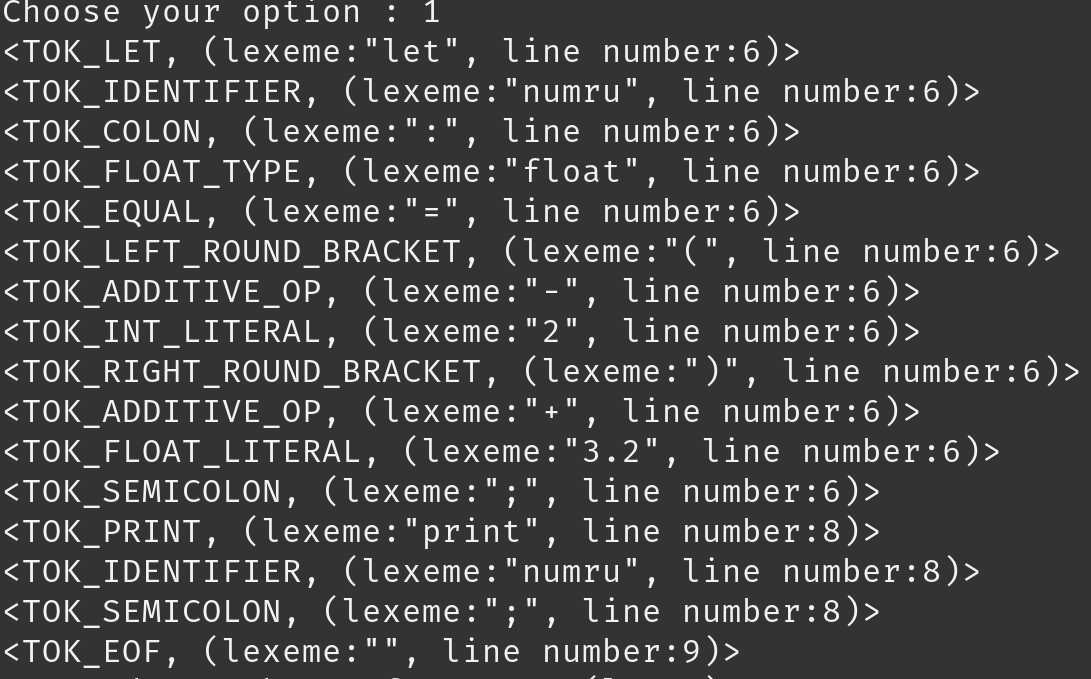
\includegraphics[scale=0.50]{Task1/output/tokenOutput1.png}
    \caption{Tokens for Program 1}
    \label{fig:tokens for program 1}
\end{figure}
    \item A program which prints 1,2,...,10 using a for loop and a while loop
\begin{lstlisting}[basicstyle=\tiny,caption=Program 2]
//a function must always return
fn forLoop()->bool{
	for(let i:int=1;i<=10;i=i+1){
		print i;
	}
	return true;
}
fn whileLoop()->bool{
	let i:int=1;
	while(i<=10){
		print i;
		i=i+1;
	}
	return false;
}
/*
a statement cannot be a function call (see EBNF)
 we assign an identifier bool x
*/
let x:bool=forLoop();
x=whileLoop();
print(x);
\end{lstlisting}
\begin{figure}[H]
    \centering
    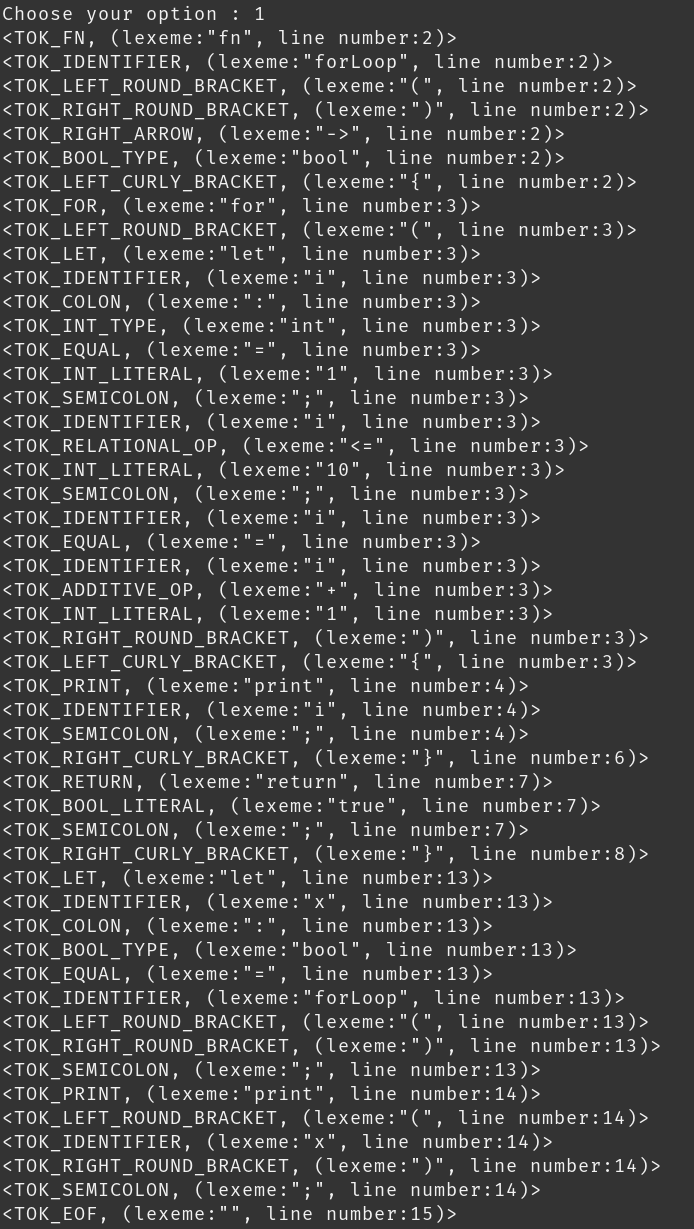
\includegraphics[scale=0.60]{Task1/output/tokenOutput2.png}
    \caption{Tokens for Program 2}
    \label{fig:tokens for program 2}
\end{figure}
\end{itemize}
{\tiny
Lexer produces expected tokens for Program 1 and Program 2. More programs were tested to ensure that the lexer produces the correct tokens. \textbf{Note also that comments are not considered in the output of the token list.}}